\documentclass[1p]{elsarticle_modified}
%\bibliographystyle{elsarticle-num}

%\usepackage[colorlinks]{hyperref}
%\usepackage{abbrmath_seonhwa} %\Abb, \Ascr, \Acal ,\Abf, \Afrak
\usepackage{amsfonts}
\usepackage{amssymb}
\usepackage{amsmath}
\usepackage{amsthm}
\usepackage{scalefnt}
\usepackage{amsbsy}
\usepackage{kotex}
\usepackage{caption}
\usepackage{subfig}
\usepackage{color}
\usepackage{graphicx}
\usepackage{xcolor} %% white, black, red, green, blue, cyan, magenta, yellow
\usepackage{float}
\usepackage{setspace}
\usepackage{hyperref}

\usepackage{tikz}
\usetikzlibrary{arrows}

\usepackage{multirow}
\usepackage{array} % fixed length table
\usepackage{hhline}

%%%%%%%%%%%%%%%%%%%%%
\makeatletter
\renewcommand*\env@matrix[1][\arraystretch]{%
	\edef\arraystretch{#1}%
	\hskip -\arraycolsep
	\let\@ifnextchar\new@ifnextchar
	\array{*\c@MaxMatrixCols c}}
\makeatother %https://tex.stackexchange.com/questions/14071/how-can-i-increase-the-line-spacing-in-a-matrix
%%%%%%%%%%%%%%%

\usepackage[normalem]{ulem}

\newcommand{\msout}[1]{\ifmmode\text{\sout{\ensuremath{#1}}}\else\sout{#1}\fi}
%SOURCE: \msout is \stkout macro in https://tex.stackexchange.com/questions/20609/strikeout-in-math-mode

\newcommand{\cancel}[1]{
	\ifmmode
	{\color{red}\msout{#1}}
	\else
	{\color{red}\sout{#1}}
	\fi
}

\newcommand{\add}[1]{
	{\color{blue}\uwave{#1}}
}

\newcommand{\replace}[2]{
	\ifmmode
	{\color{red}\msout{#1}}{\color{blue}\uwave{#2}}
	\else
	{\color{red}\sout{#1}}{\color{blue}\uwave{#2}}
	\fi
}

\newcommand{\Sol}{\mathcal{S}} %segment
\newcommand{\D}{D} %diagram
\newcommand{\A}{\mathcal{A}} %arc


%%%%%%%%%%%%%%%%%%%%%%%%%%%%%5 test

\def\sl{\operatorname{\textup{SL}}(2,\Cbb)}
\def\psl{\operatorname{\textup{PSL}}(2,\Cbb)}
\def\quan{\mkern 1mu \triangleright \mkern 1mu}

\theoremstyle{definition}
\newtheorem{thm}{Theorem}[section]
\newtheorem{prop}[thm]{Proposition}
\newtheorem{lem}[thm]{Lemma}
\newtheorem{ques}[thm]{Question}
\newtheorem{cor}[thm]{Corollary}
\newtheorem{defn}[thm]{Definition}
\newtheorem{exam}[thm]{Example}
\newtheorem{rmk}[thm]{Remark}
\newtheorem{alg}[thm]{Algorithm}

\newcommand{\I}{\sqrt{-1}}
\begin{document}

%\begin{frontmatter}
%
%\title{Boundary parabolic representations of knots up to 8 crossings}
%
%%% Group authors per affiliation:
%\author{Yunhi Cho} 
%\address{Department of Mathematics, University of Seoul, Seoul, Korea}
%\ead{yhcho@uos.ac.kr}
%
%
%\author{Seonhwa Kim} %\fnref{s_kim}}
%\address{Center for Geometry and Physics, Institute for Basic Science, Pohang, 37673, Korea}
%\ead{ryeona17@ibs.re.kr}
%
%\author{Hyuk Kim}
%\address{Department of Mathematical Sciences, Seoul National University, Seoul 08826, Korea}
%\ead{hyukkim@snu.ac.kr}
%
%\author{Seokbeom Yoon}
%\address{Department of Mathematical Sciences, Seoul National University, Seoul, 08826,  Korea}
%\ead{sbyoon15@snu.ac.kr}
%
%\begin{abstract}
%We find all boundary parabolic representation of knots up to 8 crossings.
%
%\end{abstract}
%\begin{keyword}
%    \MSC[2010] 57M25 
%\end{keyword}
%
%\end{frontmatter}

%\linenumbers
%\tableofcontents
%
\newcommand\colored[1]{\textcolor{white}{\rule[-0.35ex]{0.8em}{1.4ex}}\kern-0.8em\color{red} #1}%
%\newcommand\colored[1]{\textcolor{white}{ #1}\kern-2.17ex	\textcolor{white}{ #1}\kern-1.81ex	\textcolor{white}{ #1}\kern-2.15ex\color{red}#1	}

{\Large $\underline{12n_{0345}~(K12n_{0345})}$}

\setlength{\tabcolsep}{10pt}
\renewcommand{\arraystretch}{1.6}
\vspace{1cm}\begin{tabular}{m{100pt}>{\centering\arraybackslash}m{274pt}}
\multirow{5}{120pt}{
	\centering
	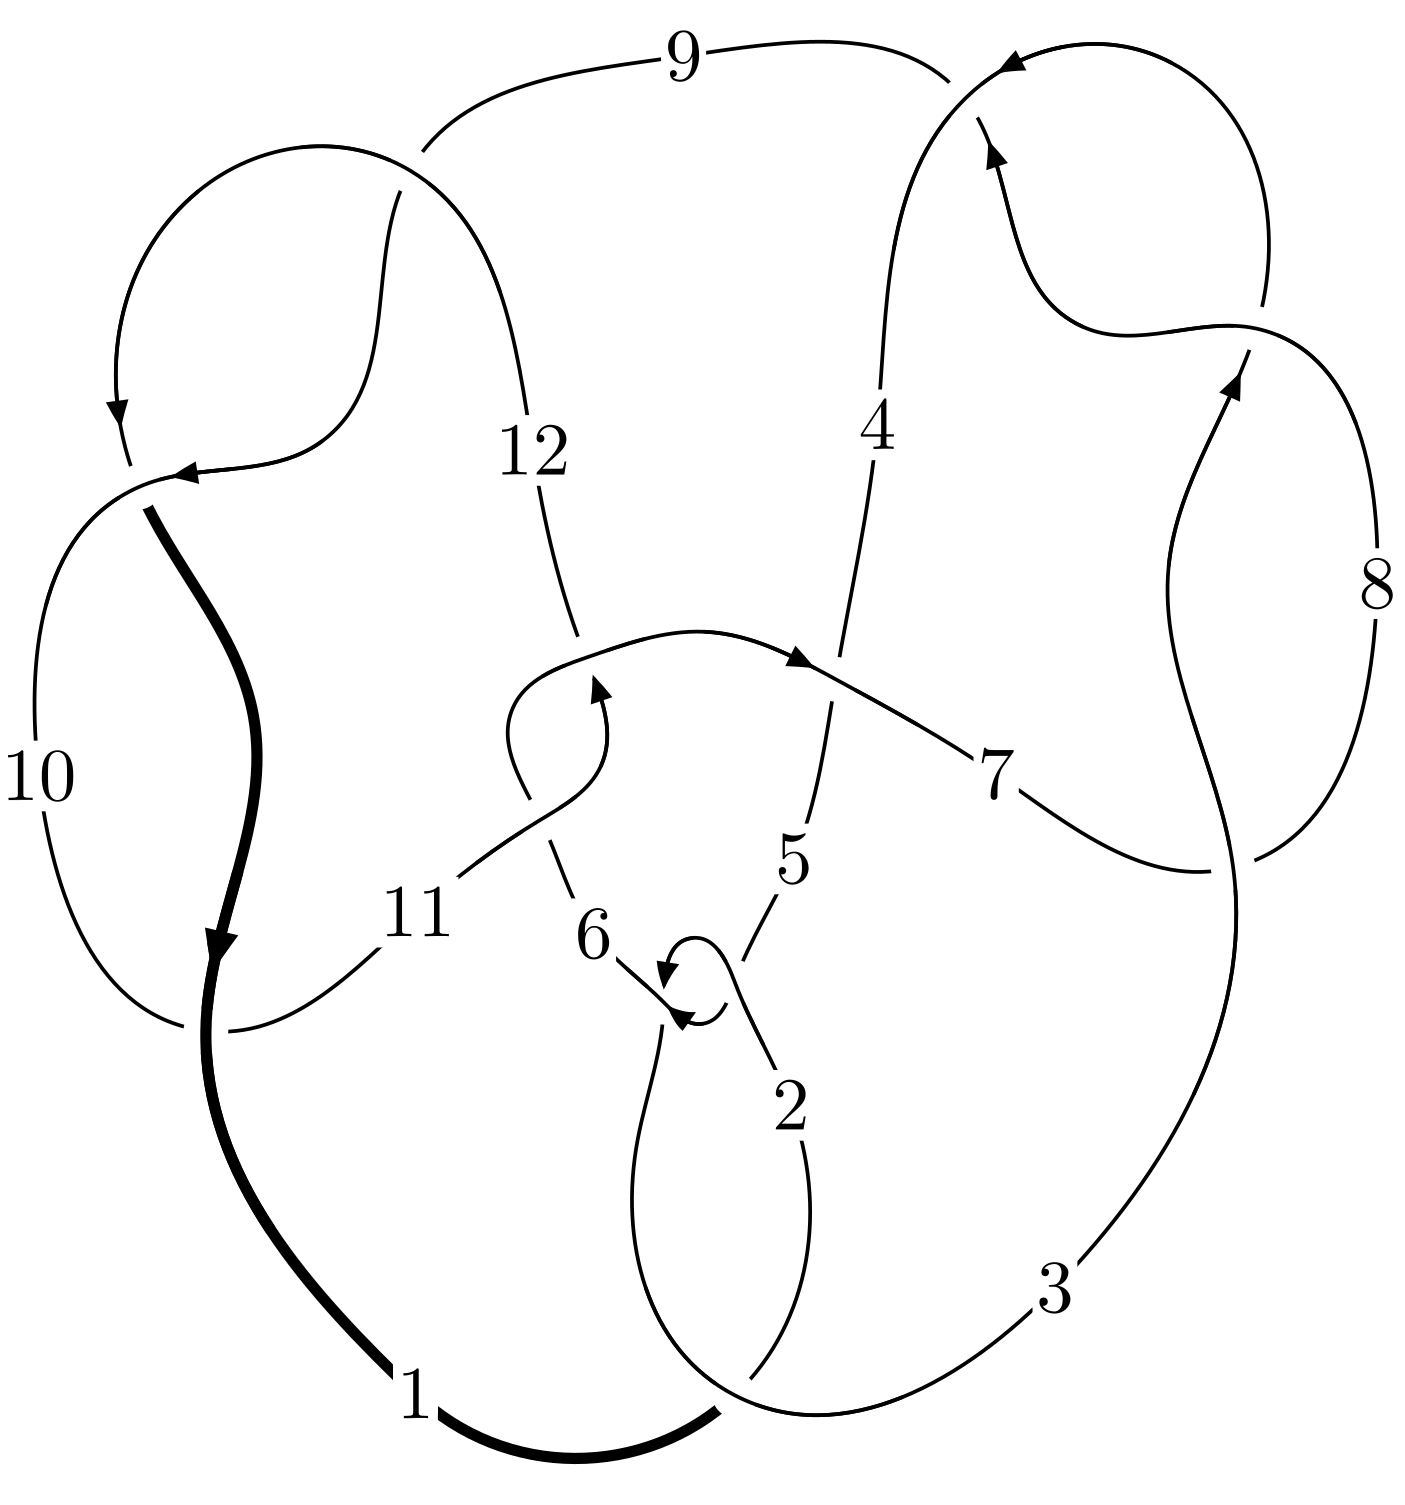
\includegraphics[width=112pt]{../../../GIT/diagram.site/Diagrams/png/2434_12n_0345.png}\\
\ \ \ A knot diagram\footnotemark}&
\allowdisplaybreaks
\textbf{Linearized knot diagam} \\
\cline{2-2}
 &
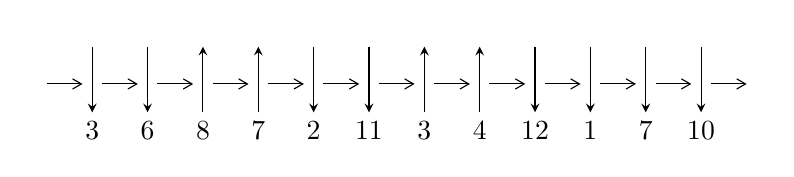
\begin{tikzpicture}[x=20pt, y=17pt]
	% nodes
	\node (C0) at (0, 0) {};
	\node (C1) at (1, 0) {};
	\node (C1U) at (1, +1) {};
	\node (C1D) at (1, -1) {3};

	\node (C2) at (2, 0) {};
	\node (C2U) at (2, +1) {};
	\node (C2D) at (2, -1) {6};

	\node (C3) at (3, 0) {};
	\node (C3U) at (3, +1) {};
	\node (C3D) at (3, -1) {8};

	\node (C4) at (4, 0) {};
	\node (C4U) at (4, +1) {};
	\node (C4D) at (4, -1) {7};

	\node (C5) at (5, 0) {};
	\node (C5U) at (5, +1) {};
	\node (C5D) at (5, -1) {2};

	\node (C6) at (6, 0) {};
	\node (C6U) at (6, +1) {};
	\node (C6D) at (6, -1) {11};

	\node (C7) at (7, 0) {};
	\node (C7U) at (7, +1) {};
	\node (C7D) at (7, -1) {3};

	\node (C8) at (8, 0) {};
	\node (C8U) at (8, +1) {};
	\node (C8D) at (8, -1) {4};

	\node (C9) at (9, 0) {};
	\node (C9U) at (9, +1) {};
	\node (C9D) at (9, -1) {12};

	\node (C10) at (10, 0) {};
	\node (C10U) at (10, +1) {};
	\node (C10D) at (10, -1) {1};

	\node (C11) at (11, 0) {};
	\node (C11U) at (11, +1) {};
	\node (C11D) at (11, -1) {7};

	\node (C12) at (12, 0) {};
	\node (C12U) at (12, +1) {};
	\node (C12D) at (12, -1) {10};
	\node (C13) at (13, 0) {};

	% arrows
	\draw[->,>={angle 60}]
	(C0) edge (C1) (C1) edge (C2) (C2) edge (C3) (C3) edge (C4) (C4) edge (C5) (C5) edge (C6) (C6) edge (C7) (C7) edge (C8) (C8) edge (C9) (C9) edge (C10) (C10) edge (C11) (C11) edge (C12) (C12) edge (C13) ;	\draw[->,>=stealth]
	(C1U) edge (C1D) (C2U) edge (C2D) (C3D) edge (C3U) (C4D) edge (C4U) (C5U) edge (C5D) (C6U) edge (C6D) (C7D) edge (C7U) (C8D) edge (C8U) (C9U) edge (C9D) (C10U) edge (C10D) (C11U) edge (C11D) (C12U) edge (C12D) ;
	\end{tikzpicture} \\
\hhline{~~} \\& 
\textbf{Solving Sequence} \\ \cline{2-2} 
 &
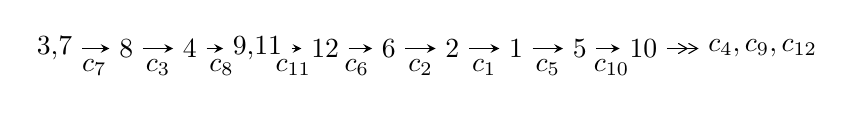
\begin{tikzpicture}[x=23pt, y=7pt]
	% node
	\node (A0) at (-1/8, 0) {3,7};
	\node (A1) at (1, 0) {8};
	\node (A2) at (2, 0) {4};
	\node (A3) at (49/16, 0) {9,11};
	\node (A4) at (33/8, 0) {12};
	\node (A5) at (41/8, 0) {6};
	\node (A6) at (49/8, 0) {2};
	\node (A7) at (57/8, 0) {1};
	\node (A8) at (65/8, 0) {5};
	\node (A9) at (73/8, 0) {10};
	\node (C1) at (1/2, -1) {$c_{7}$};
	\node (C2) at (3/2, -1) {$c_{3}$};
	\node (C3) at (5/2, -1) {$c_{8}$};
	\node (C4) at (29/8, -1) {$c_{11}$};
	\node (C5) at (37/8, -1) {$c_{6}$};
	\node (C6) at (45/8, -1) {$c_{2}$};
	\node (C7) at (53/8, -1) {$c_{1}$};
	\node (C8) at (61/8, -1) {$c_{5}$};
	\node (C9) at (69/8, -1) {$c_{10}$};
	\node (A10) at (11, 0) {$c_{4},c_{9},c_{12}$};

	% edge
	\draw[->,>=stealth]	
	(A0) edge (A1) (A1) edge (A2) (A2) edge (A3) (A3) edge (A4) (A4) edge (A5) (A5) edge (A6) (A6) edge (A7) (A7) edge (A8) (A8) edge (A9) ;
	\draw[->>,>={angle 60}]	
	(A9) edge (A10);
\end{tikzpicture} \\ 

\end{tabular} \\

\footnotetext{
The image of knot diagram is generated by the software ``\textbf{Draw programme}" developed by Andrew Bartholomew(\url{http://www.layer8.co.uk/maths/draw/index.htm\#Running-draw}), where we modified some parts for our purpose(\url{https://github.com/CATsTAILs/LinksPainter}).
}\phantom \\ \newline 
\centering \textbf{Ideals for irreducible components\footnotemark of $X_{\text{par}}$} 
 
\begin{align*}
I^u_{1}&=\langle 
-4.30590\times10^{29} u^{38}+1.40716\times10^{30} u^{37}+\cdots+3.25262\times10^{28} b-5.80343\times10^{30},\\
\phantom{I^u_{1}}&\phantom{= \langle  }-1.92426\times10^{30} u^{38}+6.35210\times10^{30} u^{37}+\cdots+3.25262\times10^{28} a-2.53835\times10^{31},\\
\phantom{I^u_{1}}&\phantom{= \langle  }u^{39}-3 u^{38}+\cdots+36 u+4\rangle \\
I^u_{2}&=\langle 
- a u+b-2 a-1,\;2 a^2- a u+2 a+2 u-3,\;u^2-2\rangle \\
\\
I^v_{1}&=\langle 
a,\;b+v+2,\;v^2+3 v+1\rangle \\
\end{align*}
\raggedright * 3 irreducible components of $\dim_{\mathbb{C}}=0$, with total 45 representations.\\
\footnotetext{All coefficients of polynomials are rational numbers. But the coefficients are sometimes approximated in decimal forms when there is not enough margin.}
\newpage
\renewcommand{\arraystretch}{1}
\centering \section*{I. $I^u_{1}= \langle -4.31\times10^{29} u^{38}+1.41\times10^{30} u^{37}+\cdots+3.25\times10^{28} b-5.80\times10^{30},\;-1.92\times10^{30} u^{38}+6.35\times10^{30} u^{37}+\cdots+3.25\times10^{28} a-2.54\times10^{31},\;u^{39}-3 u^{38}+\cdots+36 u+4 \rangle$}
\flushleft \textbf{(i) Arc colorings}\\
\begin{tabular}{m{7pt} m{180pt} m{7pt} m{180pt} }
\flushright $a_{3}=$&$\begin{pmatrix}0\\u\end{pmatrix}$ \\
\flushright $a_{7}=$&$\begin{pmatrix}1\\0\end{pmatrix}$ \\
\flushright $a_{8}=$&$\begin{pmatrix}1\\- u^2\end{pmatrix}$ \\
\flushright $a_{4}=$&$\begin{pmatrix}u\\- u^3+u\end{pmatrix}$ \\
\flushright $a_{9}=$&$\begin{pmatrix}- u^2+1\\u^4-2 u^2\end{pmatrix}$ \\
\flushright $a_{11}=$&$\begin{pmatrix}59.1604 u^{38}-195.292 u^{37}+\cdots+4436.04 u+780.403\\13.2382 u^{38}-43.2623 u^{37}+\cdots+993.748 u+178.423\end{pmatrix}$ \\
\flushright $a_{12}=$&$\begin{pmatrix}45.9221 u^{38}-152.030 u^{37}+\cdots+3442.29 u+601.980\\13.2382 u^{38}-43.2623 u^{37}+\cdots+993.748 u+178.423\end{pmatrix}$ \\
\flushright $a_{6}=$&$\begin{pmatrix}51.1260 u^{38}-169.150 u^{37}+\cdots+3814.68 u+661.729\\23.7145 u^{38}-78.2230 u^{37}+\cdots+1784.77 u+313.995\end{pmatrix}$ \\
\flushright $a_{2}=$&$\begin{pmatrix}-1.07361 u^{38}+3.79195 u^{37}+\cdots-41.8527 u+1.03040\\26.3378 u^{38}-87.1349 u^{37}+\cdots+1988.06 u+348.765\end{pmatrix}$ \\
\flushright $a_{1}=$&$\begin{pmatrix}-1.07361 u^{38}+3.79195 u^{37}+\cdots-41.8527 u+1.03040\\26.7461 u^{38}-88.2756 u^{37}+\cdots+2004.32 u+351.049\end{pmatrix}$ \\
\flushright $a_{5}=$&$\begin{pmatrix}- u^3+2 u\\- u^3+u\end{pmatrix}$ \\
\flushright $a_{10}=$&$\begin{pmatrix}7.08403 u^{38}-23.4120 u^{37}+\cdots+528.155 u+95.4828\\-26.7461 u^{38}+88.2756 u^{37}+\cdots-2004.32 u-351.049\end{pmatrix}$\\&\end{tabular}
\flushleft \textbf{(ii) Obstruction class $= -1$}\\~\\
\flushleft \textbf{(iii) Cusp Shapes $= -56.2608 u^{38}+183.733 u^{37}+\cdots-4395.07 u-821.737$}\\~\\
\newpage\renewcommand{\arraystretch}{1}
\flushleft \textbf{(iv) u-Polynomials at the component}\newline \\
\begin{tabular}{m{50pt}|m{274pt}}
Crossings & \hspace{64pt}u-Polynomials at each crossing \\
\hline $$\begin{aligned}c_{1}\end{aligned}$$&$\begin{aligned}
&u^{39}+15 u^{38}+\cdots+5679 u+81
\end{aligned}$\\
\hline $$\begin{aligned}c_{2},c_{5}\end{aligned}$$&$\begin{aligned}
&u^{39}+3 u^{38}+\cdots-45 u+9
\end{aligned}$\\
\hline $$\begin{aligned}c_{3},c_{7},c_{8}\end{aligned}$$&$\begin{aligned}
&u^{39}-3 u^{38}+\cdots+36 u+4
\end{aligned}$\\
\hline $$\begin{aligned}c_{4}\end{aligned}$$&$\begin{aligned}
&u^{39}+9 u^{38}+\cdots-12340 u-380
\end{aligned}$\\
\hline $$\begin{aligned}c_{6},c_{11}\end{aligned}$$&$\begin{aligned}
&u^{39}-2 u^{38}+\cdots-10 u+1
\end{aligned}$\\
\hline $$\begin{aligned}c_{9},c_{10},c_{12}\end{aligned}$$&$\begin{aligned}
&u^{39}-4 u^{38}+\cdots-6 u-1
\end{aligned}$\\
\hline
\end{tabular}\\~\\
\newpage\renewcommand{\arraystretch}{1}
\flushleft \textbf{(v) Riley Polynomials at the component}\newline \\
\begin{tabular}{m{50pt}|m{274pt}}
Crossings & \hspace{64pt}Riley Polynomials at each crossing \\
\hline $$\begin{aligned}c_{1}\end{aligned}$$&$\begin{aligned}
&y^{39}+25 y^{38}+\cdots+19679031 y-6561
\end{aligned}$\\
\hline $$\begin{aligned}c_{2},c_{5}\end{aligned}$$&$\begin{aligned}
&y^{39}-15 y^{38}+\cdots+5679 y-81
\end{aligned}$\\
\hline $$\begin{aligned}c_{3},c_{7},c_{8}\end{aligned}$$&$\begin{aligned}
&y^{39}-49 y^{38}+\cdots+560 y-16
\end{aligned}$\\
\hline $$\begin{aligned}c_{4}\end{aligned}$$&$\begin{aligned}
&y^{39}-109 y^{38}+\cdots+28757360 y-144400
\end{aligned}$\\
\hline $$\begin{aligned}c_{6},c_{11}\end{aligned}$$&$\begin{aligned}
&y^{39}-6 y^{38}+\cdots+46 y-1
\end{aligned}$\\
\hline $$\begin{aligned}c_{9},c_{10},c_{12}\end{aligned}$$&$\begin{aligned}
&y^{39}-30 y^{38}+\cdots+38 y-1
\end{aligned}$\\
\hline
\end{tabular}\\~\\
\newpage\flushleft \textbf{(vi) Complex Volumes and Cusp Shapes}
$$\begin{array}{c|c|c}  
\text{Solutions to }I^u_{1}& \I (\text{vol} + \sqrt{-1}CS) & \text{Cusp shape}\\
 \hline 
\begin{aligned}
u &= -0.278366 + 0.955359 I \\
a &= -0.591023 + 0.828865 I \\
b &= -0.623478 + 0.614458 I\end{aligned}
 & -3.35402 + 4.18126 I & -7.78277 - 6.99514 I \\ \hline\begin{aligned}
u &= -0.278366 - 0.955359 I \\
a &= -0.591023 - 0.828865 I \\
b &= -0.623478 - 0.614458 I\end{aligned}
 & -3.35402 - 4.18126 I & -7.78277 + 6.99514 I \\ \hline\begin{aligned}
u &= -0.887627 + 0.471243 I \\
a &= -1.50907 + 0.17598 I \\
b &= -0.886394 - 0.797483 I\end{aligned}
 & \phantom{-}2.35149 - 5.07575 I & -1.77054 + 6.40036 I \\ \hline\begin{aligned}
u &= -0.887627 - 0.471243 I \\
a &= -1.50907 - 0.17598 I \\
b &= -0.886394 + 0.797483 I\end{aligned}
 & \phantom{-}2.35149 + 5.07575 I & -1.77054 - 6.40036 I \\ \hline\begin{aligned}
u &= -0.957964\phantom{ +0.000000I} \\
a &= -0.302923\phantom{ +0.000000I} \\
b &= \phantom{-}1.25836\phantom{ +0.000000I}\end{aligned}
 & -8.12538\phantom{ +0.000000I} & -10.0210\phantom{ +0.000000I} \\ \hline\begin{aligned}
u &= \phantom{-}1.065650 + 0.085902 I \\
a &= -0.718491 + 0.083392 I \\
b &= -0.515563 + 0.600875 I\end{aligned}
 & \phantom{-}2.77568 - 0.03264 I & \phantom{-0.000000 } 0 \\ \hline\begin{aligned}
u &= \phantom{-}1.065650 - 0.085902 I \\
a &= -0.718491 - 0.083392 I \\
b &= -0.515563 - 0.600875 I\end{aligned}
 & \phantom{-}2.77568 + 0.03264 I & \phantom{-0.000000 } 0 \\ \hline\begin{aligned}
u &= -0.796295 + 0.736026 I \\
a &= \phantom{-}1.42339 + 0.01369 I \\
b &= \phantom{-}0.950413 + 0.884348 I\end{aligned}
 & -1.74573 - 9.69427 I & \phantom{-0.000000 -}0. + 8.10788 I \\ \hline\begin{aligned}
u &= -0.796295 - 0.736026 I \\
a &= \phantom{-}1.42339 - 0.01369 I \\
b &= \phantom{-}0.950413 - 0.884348 I\end{aligned}
 & -1.74573 + 9.69427 I & \phantom{-0.000000 } 0. - 8.10788 I \\ \hline\begin{aligned}
u &= \phantom{-}0.851097 + 0.768811 I \\
a &= \phantom{-}0.636558 - 0.270946 I \\
b &= \phantom{-}0.379215 - 0.675835 I\end{aligned}
 & \phantom{-}0.64343 + 2.93674 I & \phantom{-0.000000 } 0\\
 \hline 
 \end{array}$$\newpage$$\begin{array}{c|c|c}  
\text{Solutions to }I^u_{1}& \I (\text{vol} + \sqrt{-1}CS) & \text{Cusp shape}\\
 \hline 
\begin{aligned}
u &= \phantom{-}0.851097 - 0.768811 I \\
a &= \phantom{-}0.636558 + 0.270946 I \\
b &= \phantom{-}0.379215 + 0.675835 I\end{aligned}
 & \phantom{-}0.64343 - 2.93674 I & \phantom{-0.000000 } 0 \\ \hline\begin{aligned}
u &= \phantom{-}0.756459 + 0.321115 I \\
a &= \phantom{-}0.848073 + 0.323450 I \\
b &= \phantom{-}0.687338 + 0.927457 I\end{aligned}
 & -1.16384 + 3.37058 I & -4.85431 - 4.93903 I \\ \hline\begin{aligned}
u &= \phantom{-}0.756459 - 0.321115 I \\
a &= \phantom{-}0.848073 - 0.323450 I \\
b &= \phantom{-}0.687338 - 0.927457 I\end{aligned}
 & -1.16384 - 3.37058 I & -4.85431 + 4.93903 I \\ \hline\begin{aligned}
u &= -0.729654 + 0.114009 I \\
a &= \phantom{-}1.94616 - 0.30625 I \\
b &= \phantom{-}0.877049 + 0.529169 I\end{aligned}
 & -0.720527 - 0.677496 I & -4.45492 + 3.52872 I \\ \hline\begin{aligned}
u &= -0.729654 - 0.114009 I \\
a &= \phantom{-}1.94616 + 0.30625 I \\
b &= \phantom{-}0.877049 - 0.529169 I\end{aligned}
 & -0.720527 + 0.677496 I & -4.45492 - 3.52872 I \\ \hline\begin{aligned}
u &= \phantom{-}1.36027\phantom{ +0.000000I} \\
a &= -1.02723\phantom{ +0.000000I} \\
b &= -0.392618\phantom{ +0.000000I}\end{aligned}
 & \phantom{-}3.15342\phantom{ +0.000000I} & \phantom{-0.000000 } 0 \\ \hline\begin{aligned}
u &= \phantom{-}0.025858 + 0.596227 I \\
a &= \phantom{-}1.28935 - 0.78910 I \\
b &= \phantom{-}0.476410 - 0.516668 I\end{aligned}
 & -0.39053 + 1.36769 I & -3.78544 - 4.37417 I \\ \hline\begin{aligned}
u &= \phantom{-}0.025858 - 0.596227 I \\
a &= \phantom{-}1.28935 + 0.78910 I \\
b &= \phantom{-}0.476410 + 0.516668 I\end{aligned}
 & -0.39053 - 1.36769 I & -3.78544 + 4.37417 I \\ \hline\begin{aligned}
u &= -1.42742\phantom{ +0.000000I} \\
a &= -10.9292\phantom{ +0.000000I} \\
b &= -0.157920\phantom{ +0.000000I}\end{aligned}
 & \phantom{-}1.67196\phantom{ +0.000000I} & \phantom{-0.000000 } 0 \\ \hline\begin{aligned}
u &= \phantom{-}1.47236\phantom{ +0.000000I} \\
a &= \phantom{-}0.751761\phantom{ +0.000000I} \\
b &= \phantom{-}1.74885\phantom{ +0.000000I}\end{aligned}
 & -4.21706\phantom{ +0.000000I} & \phantom{-0.000000 } 0\\
 \hline 
 \end{array}$$\newpage$$\begin{array}{c|c|c}  
\text{Solutions to }I^u_{1}& \I (\text{vol} + \sqrt{-1}CS) & \text{Cusp shape}\\
 \hline 
\begin{aligned}
u &= \phantom{-}0.111960 + 0.411759 I \\
a &= -4.18092 - 0.61496 I \\
b &= -0.394904 + 0.488828 I\end{aligned}
 & -3.05808 - 0.73206 I & -13.3386 - 6.5570 I \\ \hline\begin{aligned}
u &= \phantom{-}0.111960 - 0.411759 I \\
a &= -4.18092 + 0.61496 I \\
b &= -0.394904 - 0.488828 I\end{aligned}
 & -3.05808 + 0.73206 I & -13.3386 + 6.5570 I \\ \hline\begin{aligned}
u &= \phantom{-}1.64569 + 0.02330 I \\
a &= -0.940304 - 0.261465 I \\
b &= -1.33024 + 0.90609 I\end{aligned}
 & \phantom{-}7.65877 + 1.14141 I & \phantom{-0.000000 } 0 \\ \hline\begin{aligned}
u &= \phantom{-}1.64569 - 0.02330 I \\
a &= -0.940304 + 0.261465 I \\
b &= -1.33024 - 0.90609 I\end{aligned}
 & \phantom{-}7.65877 - 1.14141 I & \phantom{-0.000000 } 0 \\ \hline\begin{aligned}
u &= -1.64517 + 0.08077 I \\
a &= -0.403452 - 0.032549 I \\
b &= -0.98617 + 1.32010 I\end{aligned}
 & \phantom{-}7.20723 - 4.84674 I & \phantom{-0.000000 } 0 \\ \hline\begin{aligned}
u &= -1.64517 - 0.08077 I \\
a &= -0.403452 + 0.032549 I \\
b &= -0.98617 - 1.32010 I\end{aligned}
 & \phantom{-}7.20723 + 4.84674 I & \phantom{-0.000000 } 0 \\ \hline\begin{aligned}
u &= \phantom{-}1.65274 + 0.23220 I \\
a &= -1.008000 - 0.471693 I \\
b &= -1.18235 + 1.09377 I\end{aligned}
 & \phantom{-}6.4748 + 13.4066 I & \phantom{-0.000000 } 0 \\ \hline\begin{aligned}
u &= \phantom{-}1.65274 - 0.23220 I \\
a &= -1.008000 + 0.471693 I \\
b &= -1.18235 - 1.09377 I\end{aligned}
 & \phantom{-}6.4748 - 13.4066 I & \phantom{-0.000000 } 0 \\ \hline\begin{aligned}
u &= \phantom{-}1.66262 + 0.24913 I \\
a &= -0.241455 - 0.016965 I \\
b &= -0.136254 + 0.574075 I\end{aligned}
 & \phantom{-}2.81425 + 0.97653 I & \phantom{-0.000000 } 0 \\ \hline\begin{aligned}
u &= \phantom{-}1.66262 - 0.24913 I \\
a &= -0.241455 + 0.016965 I \\
b &= -0.136254 - 0.574075 I\end{aligned}
 & \phantom{-}2.81425 - 0.97653 I & \phantom{-0.000000 } 0\\
 \hline 
 \end{array}$$\newpage$$\begin{array}{c|c|c}  
\text{Solutions to }I^u_{1}& \I (\text{vol} + \sqrt{-1}CS) & \text{Cusp shape}\\
 \hline 
\begin{aligned}
u &= -0.315278\phantom{ +0.000000I} \\
a &= \phantom{-}4.23572\phantom{ +0.000000I} \\
b &= -0.575388\phantom{ +0.000000I}\end{aligned}
 & -2.39339\phantom{ +0.000000I} & \phantom{-}9.22220\phantom{ +0.000000I} \\ \hline\begin{aligned}
u &= \phantom{-}1.67924 + 0.13585 I \\
a &= \phantom{-}0.987276 + 0.371552 I \\
b &= \phantom{-}1.25098 - 1.02158 I\end{aligned}
 & \phantom{-}11.24360 + 7.46891 I & \phantom{-0.000000 } 0 \\ \hline\begin{aligned}
u &= \phantom{-}1.67924 - 0.13585 I \\
a &= \phantom{-}0.987276 - 0.371552 I \\
b &= \phantom{-}1.25098 + 1.02158 I\end{aligned}
 & \phantom{-}11.24360 - 7.46891 I & \phantom{-0.000000 } 0 \\ \hline\begin{aligned}
u &= -0.301204\phantom{ +0.000000I} \\
a &= -2.36999\phantom{ +0.000000I} \\
b &= -1.68053\phantom{ +0.000000I}\end{aligned}
 & -10.3072\phantom{ +0.000000I} & \phantom{-}10.7730\phantom{ +0.000000I} \\ \hline\begin{aligned}
u &= -1.69258 + 0.19776 I \\
a &= -0.675700 + 0.148591 I \\
b &= -0.787702 - 1.170530 I\end{aligned}
 & \phantom{-}9.38751 - 6.54529 I & \phantom{-0.000000 } 0 \\ \hline\begin{aligned}
u &= -1.69258 - 0.19776 I \\
a &= -0.675700 - 0.148591 I \\
b &= -0.787702 + 1.170530 I\end{aligned}
 & \phantom{-}9.38751 + 6.54529 I & \phantom{-0.000000 } 0 \\ \hline\begin{aligned}
u &= -1.70589 + 0.04672 I \\
a &= \phantom{-}0.538540 - 0.089371 I \\
b &= \phantom{-}0.85440 + 1.24646 I\end{aligned}
 & \phantom{-}12.52260 - 0.71174 I & \phantom{-0.000000 } 0 \\ \hline\begin{aligned}
u &= -1.70589 - 0.04672 I \\
a &= \phantom{-}0.538540 + 0.089371 I \\
b &= \phantom{-}0.85440 - 1.24646 I\end{aligned}
 & \phantom{-}12.52260 + 0.71174 I & \phantom{-0.000000 } 0 \\ \hline\begin{aligned}
u &= -0.262239\phantom{ +0.000000I} \\
a &= \phantom{-}2.84003\phantom{ +0.000000I} \\
b &= \phantom{-}0.533756\phantom{ +0.000000I}\end{aligned}
 & -1.18388\phantom{ +0.000000I} & -7.92960\phantom{ +0.000000I}\\
 \hline 
 \end{array}$$\newpage\newpage\renewcommand{\arraystretch}{1}
\centering \section*{II. $I^u_{2}= \langle - a u+b-2 a-1,\;2 a^2- a u+2 a+2 u-3,\;u^2-2 \rangle$}
\flushleft \textbf{(i) Arc colorings}\\
\begin{tabular}{m{7pt} m{180pt} m{7pt} m{180pt} }
\flushright $a_{3}=$&$\begin{pmatrix}0\\u\end{pmatrix}$ \\
\flushright $a_{7}=$&$\begin{pmatrix}1\\0\end{pmatrix}$ \\
\flushright $a_{8}=$&$\begin{pmatrix}1\\-2\end{pmatrix}$ \\
\flushright $a_{4}=$&$\begin{pmatrix}u\\- u\end{pmatrix}$ \\
\flushright $a_{9}=$&$\begin{pmatrix}-1\\0\end{pmatrix}$ \\
\flushright $a_{11}=$&$\begin{pmatrix}a\\a u+2 a+1\end{pmatrix}$ \\
\flushright $a_{12}=$&$\begin{pmatrix}- a u- a-1\\a u+2 a+1\end{pmatrix}$ \\
\flushright $a_{6}=$&$\begin{pmatrix}\frac{1}{2} u\\- a u-2 a-2\end{pmatrix}$ \\
\flushright $a_{2}=$&$\begin{pmatrix}\frac{1}{2} u\\- a u-2 a+u-2\end{pmatrix}$ \\
\flushright $a_{1}=$&$\begin{pmatrix}\frac{1}{2} u\\- a u-2 a-2\end{pmatrix}$ \\
\flushright $a_{5}=$&$\begin{pmatrix}0\\- u\end{pmatrix}$ \\
\flushright $a_{10}=$&$\begin{pmatrix}a u+2 a+\frac{1}{2} u\\- a u-2 a-2\end{pmatrix}$\\&\end{tabular}
\flushleft \textbf{(ii) Obstruction class $= 1$}\\~\\
\flushleft \textbf{(iii) Cusp Shapes $= -8$}\\~\\
\newpage\renewcommand{\arraystretch}{1}
\flushleft \textbf{(iv) u-Polynomials at the component}\newline \\
\begin{tabular}{m{50pt}|m{274pt}}
Crossings & \hspace{64pt}u-Polynomials at each crossing \\
\hline $$\begin{aligned}c_{1},c_{5}\end{aligned}$$&$\begin{aligned}
&(u-1)^4
\end{aligned}$\\
\hline $$\begin{aligned}c_{2}\end{aligned}$$&$\begin{aligned}
&(u+1)^4
\end{aligned}$\\
\hline $$\begin{aligned}c_{3},c_{4},c_{7}\\c_{8}\end{aligned}$$&$\begin{aligned}
&(u^2-2)^2
\end{aligned}$\\
\hline $$\begin{aligned}c_{6},c_{12}\end{aligned}$$&$\begin{aligned}
&(u^2- u-1)^2
\end{aligned}$\\
\hline $$\begin{aligned}c_{9},c_{10},c_{11}\end{aligned}$$&$\begin{aligned}
&(u^2+u-1)^2
\end{aligned}$\\
\hline
\end{tabular}\\~\\
\newpage\renewcommand{\arraystretch}{1}
\flushleft \textbf{(v) Riley Polynomials at the component}\newline \\
\begin{tabular}{m{50pt}|m{274pt}}
Crossings & \hspace{64pt}Riley Polynomials at each crossing \\
\hline $$\begin{aligned}c_{1},c_{2},c_{5}\end{aligned}$$&$\begin{aligned}
&(y-1)^4
\end{aligned}$\\
\hline $$\begin{aligned}c_{3},c_{4},c_{7}\\c_{8}\end{aligned}$$&$\begin{aligned}
&(y-2)^4
\end{aligned}$\\
\hline $$\begin{aligned}c_{6},c_{9},c_{10}\\c_{11},c_{12}\end{aligned}$$&$\begin{aligned}
&(y^2-3 y+1)^2
\end{aligned}$\\
\hline
\end{tabular}\\~\\
\newpage\flushleft \textbf{(vi) Complex Volumes and Cusp Shapes}
$$\begin{array}{c|c|c}  
\text{Solutions to }I^u_{2}& \I (\text{vol} + \sqrt{-1}CS) & \text{Cusp shape}\\
 \hline 
\begin{aligned}
u &= \phantom{-}1.41421\phantom{ +0.000000I} \\
a &= -0.473911\phantom{ +0.000000I} \\
b &= -0.618034\phantom{ +0.000000I}\end{aligned}
 & \phantom{-}2.30291\phantom{ +0.000000I} & -8.00000\phantom{ +0.000000I} \\ \hline\begin{aligned}
u &= \phantom{-}1.41421\phantom{ +0.000000I} \\
a &= \phantom{-}0.181018\phantom{ +0.000000I} \\
b &= \phantom{-}1.61803\phantom{ +0.000000I}\end{aligned}
 & -5.59278\phantom{ +0.000000I} & -8.00000\phantom{ +0.000000I} \\ \hline\begin{aligned}
u &= -1.41421\phantom{ +0.000000I} \\
a &= \phantom{-}1.05505\phantom{ +0.000000I} \\
b &= \phantom{-}1.61803\phantom{ +0.000000I}\end{aligned}
 & -5.59278\phantom{ +0.000000I} & -8.00000\phantom{ +0.000000I} \\ \hline\begin{aligned}
u &= -1.41421\phantom{ +0.000000I} \\
a &= -2.76216\phantom{ +0.000000I} \\
b &= -0.618034\phantom{ +0.000000I}\end{aligned}
 & \phantom{-}2.30291\phantom{ +0.000000I} & -8.00000\phantom{ +0.000000I}\\
 \hline 
 \end{array}$$\newpage\newpage\renewcommand{\arraystretch}{1}
\centering \section*{III. $I^v_{1}= \langle a,\;b+v+2,\;v^2+3 v+1 \rangle$}
\flushleft \textbf{(i) Arc colorings}\\
\begin{tabular}{m{7pt} m{180pt} m{7pt} m{180pt} }
\flushright $a_{3}=$&$\begin{pmatrix}v\\0\end{pmatrix}$ \\
\flushright $a_{7}=$&$\begin{pmatrix}1\\0\end{pmatrix}$ \\
\flushright $a_{8}=$&$\begin{pmatrix}1\\0\end{pmatrix}$ \\
\flushright $a_{4}=$&$\begin{pmatrix}v\\0\end{pmatrix}$ \\
\flushright $a_{9}=$&$\begin{pmatrix}1\\0\end{pmatrix}$ \\
\flushright $a_{11}=$&$\begin{pmatrix}0\\- v-2\end{pmatrix}$ \\
\flushright $a_{12}=$&$\begin{pmatrix}v+2\\- v-2\end{pmatrix}$ \\
\flushright $a_{6}=$&$\begin{pmatrix}1\\- v-3\end{pmatrix}$ \\
\flushright $a_{2}=$&$\begin{pmatrix}v-1\\v+3\end{pmatrix}$ \\
\flushright $a_{1}=$&$\begin{pmatrix}-1\\v+3\end{pmatrix}$ \\
\flushright $a_{5}=$&$\begin{pmatrix}v\\0\end{pmatrix}$ \\
\flushright $a_{10}=$&$\begin{pmatrix}- v-2\\v+3\end{pmatrix}$\\&\end{tabular}
\flushleft \textbf{(ii) Obstruction class $= 1$}\\~\\
\flushleft \textbf{(iii) Cusp Shapes $= -26$}\\~\\
\newpage\renewcommand{\arraystretch}{1}
\flushleft \textbf{(iv) u-Polynomials at the component}\newline \\
\begin{tabular}{m{50pt}|m{274pt}}
Crossings & \hspace{64pt}u-Polynomials at each crossing \\
\hline $$\begin{aligned}c_{1},c_{2}\end{aligned}$$&$\begin{aligned}
&(u-1)^2
\end{aligned}$\\
\hline $$\begin{aligned}c_{3},c_{4},c_{7}\\c_{8}\end{aligned}$$&$\begin{aligned}
&u^2
\end{aligned}$\\
\hline $$\begin{aligned}c_{5}\end{aligned}$$&$\begin{aligned}
&(u+1)^2
\end{aligned}$\\
\hline $$\begin{aligned}c_{6},c_{9},c_{10}\end{aligned}$$&$\begin{aligned}
&u^2+u-1
\end{aligned}$\\
\hline $$\begin{aligned}c_{11},c_{12}\end{aligned}$$&$\begin{aligned}
&u^2- u-1
\end{aligned}$\\
\hline
\end{tabular}\\~\\
\newpage\renewcommand{\arraystretch}{1}
\flushleft \textbf{(v) Riley Polynomials at the component}\newline \\
\begin{tabular}{m{50pt}|m{274pt}}
Crossings & \hspace{64pt}Riley Polynomials at each crossing \\
\hline $$\begin{aligned}c_{1},c_{2},c_{5}\end{aligned}$$&$\begin{aligned}
&(y-1)^2
\end{aligned}$\\
\hline $$\begin{aligned}c_{3},c_{4},c_{7}\\c_{8}\end{aligned}$$&$\begin{aligned}
&y^2
\end{aligned}$\\
\hline $$\begin{aligned}c_{6},c_{9},c_{10}\\c_{11},c_{12}\end{aligned}$$&$\begin{aligned}
&y^2-3 y+1
\end{aligned}$\\
\hline
\end{tabular}\\~\\
\newpage\flushleft \textbf{(vi) Complex Volumes and Cusp Shapes}
$$\begin{array}{c|c|c}  
\text{Solutions to }I^v_{1}& \I (\text{vol} + \sqrt{-1}CS) & \text{Cusp shape}\\
 \hline 
\begin{aligned}
v &= -0.381966\phantom{ +0.000000I} \\
a &= \phantom{-0.000000 } 0 \\
b &= -1.61803\phantom{ +0.000000I}\end{aligned}
 & -10.5276\phantom{ +0.000000I} & -26.0000\phantom{ +0.000000I} \\ \hline\begin{aligned}
v &= -2.61803\phantom{ +0.000000I} \\
a &= \phantom{-0.000000 } 0 \\
b &= \phantom{-}0.618034\phantom{ +0.000000I}\end{aligned}
 & -2.63189\phantom{ +0.000000I} & -26.0000\phantom{ +0.000000I}\\
 \hline 
 \end{array}$$\newpage
\newpage\renewcommand{\arraystretch}{1}
\centering \section*{ IV. u-Polynomials}
\begin{tabular}{m{50pt}|m{274pt}}
Crossings & \hspace{64pt}u-Polynomials at each crossing \\
\hline $$\begin{aligned}c_{1}\end{aligned}$$&$\begin{aligned}
&((u-1)^6)(u^{39}+15 u^{38}+\cdots+5679 u+81)
\end{aligned}$\\
\hline $$\begin{aligned}c_{2}\end{aligned}$$&$\begin{aligned}
&((u-1)^2)(u+1)^4(u^{39}+3 u^{38}+\cdots-45 u+9)
\end{aligned}$\\
\hline $$\begin{aligned}c_{3},c_{7},c_{8}\end{aligned}$$&$\begin{aligned}
&u^2(u^2-2)^2(u^{39}-3 u^{38}+\cdots+36 u+4)
\end{aligned}$\\
\hline $$\begin{aligned}c_{4}\end{aligned}$$&$\begin{aligned}
&u^2(u^2-2)^2(u^{39}+9 u^{38}+\cdots-12340 u-380)
\end{aligned}$\\
\hline $$\begin{aligned}c_{5}\end{aligned}$$&$\begin{aligned}
&((u-1)^4)(u+1)^2(u^{39}+3 u^{38}+\cdots-45 u+9)
\end{aligned}$\\
\hline $$\begin{aligned}c_{6}\end{aligned}$$&$\begin{aligned}
&((u^2- u-1)^2)(u^2+u-1)(u^{39}-2 u^{38}+\cdots-10 u+1)
\end{aligned}$\\
\hline $$\begin{aligned}c_{9},c_{10}\end{aligned}$$&$\begin{aligned}
&((u^2+u-1)^3)(u^{39}-4 u^{38}+\cdots-6 u-1)
\end{aligned}$\\
\hline $$\begin{aligned}c_{11}\end{aligned}$$&$\begin{aligned}
&(u^2- u-1)(u^2+u-1)^2(u^{39}-2 u^{38}+\cdots-10 u+1)
\end{aligned}$\\
\hline $$\begin{aligned}c_{12}\end{aligned}$$&$\begin{aligned}
&((u^2- u-1)^3)(u^{39}-4 u^{38}+\cdots-6 u-1)
\end{aligned}$\\
\hline
\end{tabular}\newpage\renewcommand{\arraystretch}{1}
\centering \section*{ V. Riley Polynomials}
\begin{tabular}{m{50pt}|m{274pt}}
Crossings & \hspace{64pt}Riley Polynomials at each crossing \\
\hline $$\begin{aligned}c_{1}\end{aligned}$$&$\begin{aligned}
&((y-1)^6)(y^{39}+25 y^{38}+\cdots+19679031 y-6561)
\end{aligned}$\\
\hline $$\begin{aligned}c_{2},c_{5}\end{aligned}$$&$\begin{aligned}
&((y-1)^6)(y^{39}-15 y^{38}+\cdots+5679 y-81)
\end{aligned}$\\
\hline $$\begin{aligned}c_{3},c_{7},c_{8}\end{aligned}$$&$\begin{aligned}
&y^2(y-2)^4(y^{39}-49 y^{38}+\cdots+560 y-16)
\end{aligned}$\\
\hline $$\begin{aligned}c_{4}\end{aligned}$$&$\begin{aligned}
&y^2(y-2)^4(y^{39}-109 y^{38}+\cdots+2.87574\times10^{7} y-144400)
\end{aligned}$\\
\hline $$\begin{aligned}c_{6},c_{11}\end{aligned}$$&$\begin{aligned}
&((y^2-3 y+1)^3)(y^{39}-6 y^{38}+\cdots+46 y-1)
\end{aligned}$\\
\hline $$\begin{aligned}c_{9},c_{10},c_{12}\end{aligned}$$&$\begin{aligned}
&((y^2-3 y+1)^3)(y^{39}-30 y^{38}+\cdots+38 y-1)
\end{aligned}$\\
\hline
\end{tabular}
\vskip 2pc
\end{document}